\documentclass[a4paper,12pt]{article} % тип документа
\usepackage[margin=1in]{geometry} % Поля

%  Русский язык
\usepackage[warn]{mathtext}
\usepackage[T2A]{fontenc}			% кодировка
\usepackage[utf8]{inputenc}			% кодировка исходного текста
\usepackage[english,russian]{babel}	% локализация и переносы
% Математика
\usepackage{amsmath,amsfonts,amssymb,amsthm,mathtools} 
\usepackage{wasysym}
%%%
\usepackage{graphicx}

\usepackage{gensymb} % знак градуса \degree

%%%% Римские цифры
\renewcommand{\thesection}{\Roman{section}.} 
\renewcommand{\thesubsection}{\roman{subsection}.}


\begin{document}
%титул
\hrule 	
\medskip
\begin{raggedright}
{\large \textbf{Отчёт по работе 2.2.1}}
\\
\medskip
{\Large Исследование взаимной диффузии газов} 
\\
\medskip
{\large Карташов Константин Б04-005}
\medskip
\hrule
\medskip
\end{raggedright}


\section{Аннотация}


\paragraph{Цель работы:} 
\begin{enumerate}
\itemsep0em
\item регистрация зависимости концентрации гелия в воздухе от времени с помощью датчиков теплопроводности при разных начальных давлениях смеси газов
\item определение коэффициента диффузии по результатам измерений
\end{enumerate}

\paragraph{В работе используются:}
\begin{itemize}
\itemsep0em
\renewcommand{\labelitemi}{$\triangleright$}
\item измерительная установка
\item форвакуумный насос 
\item баллон с газом (He)
\item манометр
\item источник питания
\item магазин сопротивлений 
\item гальванометр
\item секундомер
\end{itemize}



\medskip\hrule\medskip

\section{Теоретическая часть}

\subsection{Необходимые теоретические знания для проведения эксперимента}

\paragraph{} \textit{Диффузией} называют самопроизвольное взаимное проникновение веществ друг в друга, происходящее вследствие хаотичного теплового движения молекул. При перемешивании молекул разного сорта говорят о \textit{взаимной (концентрационной)} диффузии.

Диффузия в системе, состоящей из двух компонентов $a$ и $b$, подчиняется закону Фика: плотности потока компонентов $j_{a,b}$(количество частиц, пересекающих единичную площадку в единицу времени) пропорциональны градиентам их концентраций $\nabla n_{a, b}$, что в одномерном случае можно записать как:
\begin{equation}
j_a = -D_{ab}\frac{\partial n_a}{\partial x}, 
\;\;\; j_b = -D_{ba}\frac{\partial n_b}{\partial x}
\end{equation} 
где $D_{ab} = D_{ba} = D$ - коэффициент взаимной диффузии компонентов

В данной работе исследуется взаимная диффузия гелия и воздуха. Давление $P$ и температура $T$ в условиях опыта предполагаются неизменными: $P = (n_{He}+n_{B}k_\text{Б},\; T = const$, где $n_{He}, n_{B}$ -- концентрации диффундирующих газов. Поэтому для любых изменений концентраций справедливо $\Delta n_{B} = \Delta n_{He}$. Следовательно, достаточно ограничиться описанием диффузии одного из компонентов (остановимся на гелии)

Приведём теоретическую оценку для коэффициента диффузии. В работе концентрация гелия, как правило, мала $(n_{He}\ll n_{в})$. Кроме того, атомы гелия
существенно легче молекул, составляющих воздух $(\mu_{He}\ll\mu_{N_2},\mu_{O_2})$, значит и их средняя тепловая скорость велика по сравнению с остальными частицами. Поэтому перемешивание газов в работе можно приближенно описывать как диффузию примеси лёгких частиц гелия на практически стационарном фоне воздуха. Коэффициент диффузии в таком приближении равен:
\begin{equation}
D = \frac{1}{3}\lambda\langle v \rangle,
\end{equation}
где $\langle v \rangle = \sqrt{\dfrac{8RT}{\pi\mu}}$ -- средняя тепловая скорость частиц примеси, $\lambda = \dfrac{1}{n_0\sigma}$ -- их длина свободного пробега, $n_0$ -- концентрация рассеивающего фона, $\sigma$ -- сечение столкновения частиц примеси с частицами фона.

В общем случае необходимо учитывать диффузию каждого из
компонентов. Более подробное рассмотрение показывает, что для бинарной смеси формула (2) сохраняется, если:
\begin{enumerate}
\itemsep0em
\item Под $\lambda$ понимать величину $\lambda = \dfrac{1}{n_{\Sigma}\sigma}$, где $n_{\Sigma}=n_{He}+n_{B} = \dfrac{P}{k_{\text{Б}}T}$ -- полная концентрация частиц
\item Под $\langle v \rangle$ понимать среднюю относительную скорость частиц разных сортов.

\end{enumerate}

Таким образом, теория предсказывает, что коэффициент диффузии бинарной смеси обратно пропорционален давлению в системе, и не зависит от пропорций компонентов, что и предлагается проверить в работе экспериментально ($D\propto\frac{1}{P}$)

Для исследования взаимной диффузии используется установка, изображенная на рисунке 1. Два сосуда с примерно одинаковыми объемами $V_1 \approx V_2 \equiv V$ соединены трубкой длины l и сечения S. Сосуды заполнены смесью двух газов при одинаковом давлении, но с различной концентрацией компонентов. Вследствие взаимной диффузии концентрации каждого из компонентов в обоих сосудах с течением времени выравниваются. 

Рассмотрим этот процесс. Решение задачи упрощается, если сделать несколько допущений:
\begin{enumerate}
\itemsep0em
\item Пренебрежем объемом соединительной трубки, поскольку он мал по сравнению с объемами сосудов
\item Концентрацию газов в каждом из сосудов будем считать постоянной по всему объему сосуда
\item Предположим, что процесс выравнивания концентраций происходит в основном благодаря диффузии в трубке
\end{enumerate}
Тогда диффузионный потом в любом сечении трубки одинаков,поэтому $J = -DS(\partial n/ \partial x)$ не меняется вдоль трубки, следовательно:
\begin{equation}
J = -DS\frac{n_1 - n_2}{l}
\end{equation}
Обозначим через $\Delta n_1 \text{и} \Delta n_2$ изменения в объемах V за время $\Delta t$. Тогда $V_1\Delta n_1$ равно изменению количества компонента в объеме $V_1$, a $V_2\Delta n_2$ -- изменению этого компонента в $V_2$. Из закона сохранения вещества $V_1\Delta n_1 = -V_2\Delta n_2$. Тогда получим:
\begin{equation}
V\frac{dn_1}{dt} = -DS\frac{n_1 - n_2}{l}, \;\;\;\;\ V\frac{dn_2}{dt} = DS\frac{n_1 - n_2}{l}
\end{equation}
Вычтя уравнения друг из друга, найдем:
\begin{equation}
\frac{n_1}{dt} - \frac{dn_2}{dt} = -\frac{n_1 - n_2}{l}DS(\frac{2}{V})
\end{equation}
Интегрируя, получим:
\begin{equation}
n_1 - n_2 = (n_1 - n_2)_0 e^{(-t/\tau)}
\end{equation}
где $(n_1 - n_2)_0$ -- разность концентраций в начальный момент времени, $\tau = \dfrac{V}{2}\dfrac{l}{SD}$ -- постоянная времени процесса, определяемая геометрией установки и величиной коэффициента диффузии D.

Для проверки применимости квазистационарного течения убедимся, что время $\tau$ много больше характерного времени диффузии одной частицы вдоль трубки длиной $l$: $t_{\text{диф}} \sim \frac{l^2}{D} \ll \tau$.

 Для измерения концентраций применяются датчики теплопроводности $D_1$ и $D_2$ (см. рис. 1) и используется зависимость теплопроводности газовой смеси от её состава. Тонкая проволока радиуса $r_{\text{пр}}$, протянутая вдоль оси цилиндра радиуса $R_{\text{ц}}$, нагревается током. Тепло от проволоки к стенке цилиндра передаётся главным образом вследствие теплопроводности газа, находящегося внутри цилиндра. Количество тепла переданного стенке цилиндра в единицу времени, определяется по формуле 
\begin{equation}
Q = \varkappa \frac{2\pi L}{ln (R_{\text{ц}}/r_{\text{пр}})}(T_1-T_2)
\end{equation}
где $\varkappa$ - теплопроводность, $L$ - длина нити, $T_1, T_2$ - температуры проволочки и стенки. При $Q = const$ температура проволоки и её сопротивление определяются теплопроводностью газа и, следовательно, его составом. Для измерения разности концентраций газов используется  
мостовая схема, представленная на рисунке 2 (см. описание установки).
	 
	 При разности концентраций, равной $15\%$, поправка к линейному закону не превышает $0,5\%$, что для наших целей достаточно.
	 
 В процессе диффузии разность концентраций убывает по экспоненциальному закону. По тому же закону изменяются во времени показания гальванометра:
\begin{equation}
U = U_0e^{-t/\tau} \label{voltage}
\end{equation}
Измеряя экспериментально зависимость $U(t)$, можно получить характерное время процесса $\tau$, откуда определить коэффициент диффузии D.



\subsection{Контрольные вопросы}

\paragraph{Вопрос 1:}
Покажите, что в условиях опыта концентрацию газов можно считать постоянной по всему объёму сосуда $V_1$ (и $V_2$).

Ответ.

\paragraph{Вопрос 2:}
Почему следует ожидать, что график зависимости $D$ от $1/P$ должен иметь вид прямой линии?

Ответ.


\medskip\hrule\medskip

\section{Экспериментальная часть}

\subsection{Устройство экспериментальной установки}

\begin{figure}[h]
\begin{center}
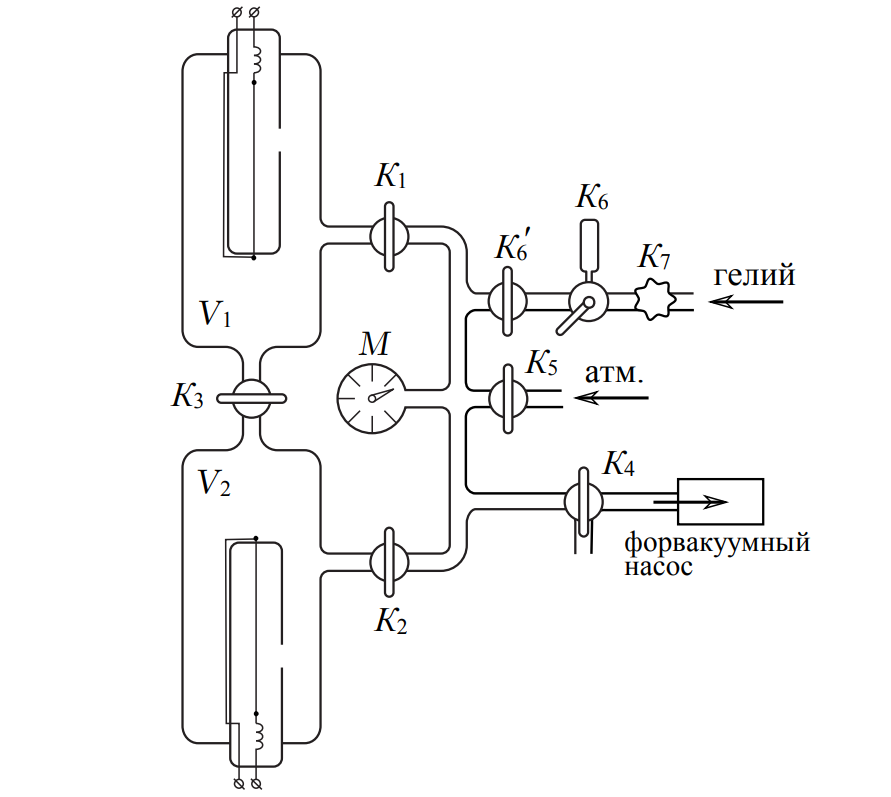
\includegraphics[width=0.5\linewidth]{ustanovka_graph.png}
\label{ris:ustanovka_1} 
\caption{Установка для исследования взаимной диффузии газов}
\end{center}
\end{figure}
\paragraph{}
Установка состоит из двух сосудов $V_1 \approx V_2 \equiv V$, соединенных краном $K_3$, форвакуумного насоса, манометра М и системы напуска гелия, включающей в себя краны $K_6, \; K'_6,\; K_7$. Дополнительный кран $K'_6$ служит для вакуумной изоляции установки от системы подачи гелия. Для подачи воздуха в установку служит кран $K_5$. Сосуды $V_1 \; \text{и} \; V_2$ и порознь и вместе можно соединять как с системой напуска гелия, так и с форвакуумным насосом. Для этого служат краны $K_1,\; K_2,\; K_4,\; K_5$. Манометр М регистрирует давление газа, до которого заполняют тот или другой сосуды. Краны $K_4,\; K_5 \; \text{и} \; K'_6$ обладают повышенной вакуумплотностью и хорошо изолируют установку от протечек.

В силу того, что в сосуд требуется подавать малое давление гелия, кран $K_6$ снабжен дозатором. Подробный разрез крана $K_6$ приведен на рисунке 3.

На рисунке 2 приведена схема электричского соединения $D_1 \; \text{и} \; D_2$ -- сопротивления проволок датчиков парциального давления, которые состовляют одно плечо моста. Второе плечо моста состовляют сопротивления $r_1, \; R_1, \; r_2, \; R_2, \; r_1 \ll R_1, \; r_2 \ll R_2, \; R_1 \; \text{и} \; R_2$ спаренные, их подвижные контакты находятся на общей оси. Оба они используются для грубой регулировки моста. Точная балансировка моста выполняется потенциометром $R$. Последовательо с гальванометром Г, стоящим в диагонали моста, поставлен магазин сопротивления $M_R$. Когда мост балансируют, магазин сопротивлений выводят на ноль. 


\begin{figure}[h]
\begin{center}
\begin{minipage}[h]{0.4\linewidth}
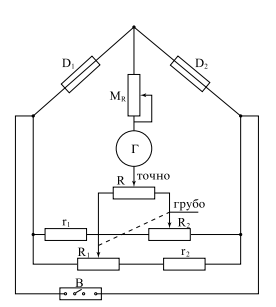
\includegraphics[width=0.8\linewidth]{bridge.png}
\label{bridge}
\caption{Мостовая схема с датчиками теплопроводности для измерения разности концентраций газов} 
\end{minipage}
\hfill
\begin{minipage}[h]{0.5\linewidth}
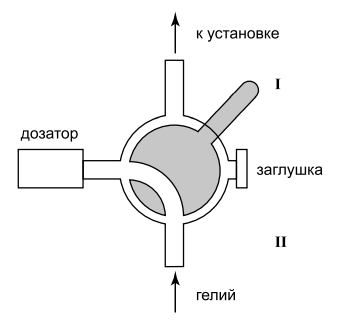
\includegraphics[width=1\linewidth]{K_6.png}
\caption{Кран $K_6$}
\end{minipage}
\end{center}
\end{figure}

\subsection{Ход работы}

\begin{enumerate}
\itemsep0em
\item Ознакомимся со схемой установки. Перепишем параметры установки: 
$$V_1 = V_2 = V = 775 \pm 10 \; \text{см}^{3}, \; \frac{L}{S} = 5,3 \pm 0.1 \; 
\text{см}^{-1}$$ 
проверим, что краны $K_4,\; K_5 \; K'_6$ закрыты перед началом откачки. 
\item Включим питание электрической схемы установки. Откроем краны $K_1$, $K_2$, $K_3$.
Поскольку манометр измеряет разность давления внутри резервуаров с атмосферным в $\frac{\text{кгс}}{\text{cм}^2}$ необходимо записать показание манометра при полностью откачанном сосуде $P_0 = 99,5 \;\dfrac{\text{кгс}}{\text{cм}^2}$ (оно равно атмосферному) и в дальнейшем постоянно вычитать из него показания прибора, тем самым будет найдено давление внутри установки.
\item Очистим установку от всех газов, которые в ней есть. Для этого откроем кран $K_4$. Включим форвакуумный насос  и соединим его с установкой, повернув ручку крана $K_5$ длинным концом рукоятки влево (на установку). Откачаем установку до давления $\approx 0.1 \; \text{торр} $, что достигается непрерывной работой насоса в течение 3–5 минут. Для прекращения откачки ручку крана $K_5$ поставим длинным концом вверх, выключим насос
\item  Напустим в установку воздух до рабочего давления (вначале $P \approx 40 \; \text{торр}$), открыв кран $K_5$, чтобы сбалансировать мост на рабочем давлении. Сбалансируем мост.
\item Заполним установку рабочей смесью согласно порядку предложенному в указании к работе: в сосуде $V_2$ должен быть воздух, а в сосуде $V_1$ — смесь воздуха с гелием.
\item Проведём измерения. Для этого откроем кран $K_3$, заснимем на видео процесс падения напряжения на гальванометре на $40 - 50\%$ Будем продолжать аналогичные измерения при различных значениях $P_\text{раб}$ в интервале $40 - 200$ торр. Результаты измерений приведены во вложении 1.
\item Для каждого из давлений построим графики, откладывая по
оси абсцисс время, а по оси ординат - логарифм от показаний гальванометра.
\end{enumerate}


\subsection{Проведение измерений}

При разных значениях $P_\Sigma$ замерим зависимость показаний вольтметра $u$ от времени, а также вычислим $\ln{u}$ для построения графика $\ln{u} (t)$. Взяв логарифм от формулы (\ref{voltage}) получим $\ln(u) = \ln(u_0) + t/\tau$. То есть коэффициент наклона графика $\alpha = 1/\tau$.

\paragraph{Измерение 1.}
Возьмём $P_\Sigma = 40$ торр. Получим зависимость показаний вольтметра от времени:

\begin{center}
\begin{tabular}{|c||c|c|c|c|c|c|c|c|c|c|c|c|}
\hline
$t$ & 5 & 10 & 15 & 20 & 25 & 30 \\ 
\hline
$v$ & 1356 & 1355 & 1344 & 1329 & 1300 & 1268 \\ 
\hline
\hline
$t$ & 35 & 40 & 45 & 50 & 55 & 60 \\ 
\hline
$v$ & 1237 & 1207 & 1180 & 1158 & 1124 & 1098 \\ 
\hline
\hline
$t$ & 65 & 70 & 75 & 80 & 85 & 90 \\ 
\hline
$v$ & 1072 & 1045 & 1028 & 997 & 969 & 946 \\ 
\hline
\hline
$t$ & 95 & 100 & 105 & 110 & 115 & 120 \\ 
\hline
$v$ & 924 & 902 & 880 & 858 & 839 & 819 \\ 
\hline
\hline
$t$ & 125 & 130 & 135 & 140 & 145 & 150 \\ 
\hline
$v$ & 799 & 778 & 759 & 741 & 722 & 705 \\ 
\hline
\hline
$t$ & 155 & 160 & 165 & 170 & 175 & 180 \\ 
\hline
$v$ & 688 & 669 & 653 & 638 & 620 & 607 \\ 
\hline
\end{tabular}
\end{center}

\paragraph{Измерение 2.}
Возьмём $P_\Sigma = 80$ торр. Получим зависимость показаний вольтметра от времени:

\begin{center}
\begin{tabular}{|c||c|c|c|c|c|c|c|c|c|c|c|c|c|}
\hline
$t$ & 5 & 10 & 15 & 20 & 25 & 30 & 35 \\ 
\hline
$v$ & 901 & 899 & 887 & 874 & 868 & 848 & 834 \\ 
\hline
\hline
$t$ & 40 & 45 & 50 & 55 & 60 & 65 & 70 \\ 
\hline
$v$ & 819 & 808 & 797 & 783 & 772 & 760 & 747 \\ 
\hline
\hline
$t$ & 75 & 80 & 85 & 90 & 95 & 100 & 105 \\ 
\hline
$v$ & 737 & 727 & 716 & 706 & 694 & 684 & 679 \\ 
\hline
\hline
$t$ & 110 & 115 & 120 & 125 & 130 & 135 & 140 \\ 
\hline
$v$ & 666 & 656 & 646 & 636 & 625 & 616 & 609 \\ 
\hline
\hline
$t$ & 145 & 150 & 155 & 160 & 165 & 170 & 175 \\ 
\hline
$v$ & 599 & 592 & 584 & 575 & 566 & 557 & 549 \\ 
\hline
\hline
$t$ & 180 & 185 & 190 & 195 & 200 & 205 & 210 \\ 
\hline
$v$ & 542 & 539 & 528 & 518 & 511 & 503 & 498 \\ 
\hline
\end{tabular}
\end{center}

\paragraph{Измерение 3.}
Возьмём $P_\Sigma = 120$ торр. Получим зависимость показаний вольтметра от времени:


\begin{center}
\begin{tabular}{|c||c|c|c|c|c|c|c|c|c|c|c|c|c|}
\hline
$t$ & 5 & 10 & 15 & 20 & 25 & 30 & 35 \\ 
\hline
$v$ & 777 & 773 & 766 & 757 & 749 & 740 & 731 \\ 
\hline
\hline
$t$ & 40 & 45 & 50 & 55 & 60 & 65 & 70 \\ 
\hline
$v$ & 723 & 714 & 706 & 699 & 692 & 685 & 677 \\ 
\hline
\hline
$t$ & 75 & 80 & 85 & 90 & 95 & 100 & 105 \\ 
\hline
$v$ & 669 & 662 & 656 & 647 & 642 & 633 & 627 \\ 
\hline
\hline
$t$ & 110 & 115 & 120 & 125 & 130 & 135 & 140 \\ 
\hline
$v$ & 622 & 614 & 607 & 603 & 596 & 589 & 586 \\ 
\hline
\hline
$t$ & 145 & 150 & 155 & 160 & 165 & 170 & 175 \\ 
\hline
$v$ & 580 & 573 & 568 & 563 & 554 & 550 & 544 \\ 
\hline
\hline
$t$ & 180 & 185 & 190 & 195 & 200 & 205 & 210 \\ 
\hline
$v$ & 539 & 534 & 528 & 525 & 520 & 516 & 508 \\ 
\hline
\end{tabular}
\end{center}


\paragraph{Измерение 4.}
Возьмём $P_\Sigma = 160$ торр. Получим зависимость показаний вольтметра от времени:

\begin{center}
\begin{tabular}{|c||c|c|c|c|c|c|c|c|c|c|c|c|c|}
\hline
$t$ & 5 & 10 & 15 & 20 & 25 & 30 & 35 \\ 
\hline
$v$ & 744 & 741 & 735 & 730 & 724 & 718 & 712 \\ 
\hline
\hline
$t$ & 40 & 45 & 50 & 55 & 60 & 65 & 70 \\ 
\hline
$v$ & 706 & 700 & 692 & 686 & 679 & 673 & 668 \\ 
\hline
\hline
$t$ & 75 & 80 & 85 & 90 & 95 & 100 & 105 \\ 
\hline
$v$ & 663 & 657 & 653 & 645 & 641 & 634 & 632 \\ 
\hline
\hline
$t$ & 110 & 115 & 120 & 125 & 130 & 135 & 140 \\ 
\hline
$v$ & 626 & 621 & 614 & 610 & 604 & 602 & 596 \\ 
\hline
\hline
$t$ & 145 & 150 & 155 & 160 & 165 & 170 & 175 \\ 
\hline
$v$ & 591 & 587 & 581 & 576 & 571 & 569 & 565 \\ 
\hline
\hline
$t$ & 180 & 185 & 190 & 195 & 200 & 205 & 210 \\ 
\hline
$v$ & 561 & 557 & 552 & 549 & 545 & 540 & 537 \\ 
\hline
\end{tabular}
\end{center}


\paragraph{Измерение 5.}
Возьмём $P_\Sigma = 200$ торр. Получим зависимость показаний вольтметра от времени:

\begin{center}
\begin{tabular}{|c||c|c|c|c|c|c|c|c|c|c|c|c|c|}
\hline
$t$ & 5 & 10 & 15 & 20 & 25 & 30 & 35 \\ 
\hline
$v$ & 616 & 616 & 613 & 607 & 604 & 598 & 591 \\ 
\hline
\hline
$t$ & 40 & 45 & 50 & 55 & 60 & 65 & 70 \\ 
\hline
$v$ & 585 & 580 & 577 & 571 & 567 & 562 & 557 \\ 
\hline
\hline
$t$ & 75 & 80 & 85 & 90 & 95 & 100 & 105 \\ 
\hline
$v$ & 554 & 550 & 547 & 540 & 537 & 533 & 530 \\ 
\hline
\hline
$t$ & 110 & 115 & 120 & 125 & 130 & 135 & 140 \\ 
\hline
$v$ & 525 & 523 & 518 & 514 & 513 & 508 & 504 \\ 
\hline
\hline
$t$ & 145 & 150 & 155 & 160 & 165 & 170 & 175 \\ 
\hline
$v$ & 502 & 498 & 494 & 494 & 490 & 487 & 483 \\ 
\hline
\hline
$t$ & 180 & 185 & 190 & 195 & 200 & 205 & 210 \\ 
\hline
$v$ & 482 & 477 & 476 & 470 & 468 & 464 & 464 \\ 
\hline
\end{tabular}
\end{center}



\medskip\hrule\medskip


\section{Выводы}

\end{document}


